\scanpage{6}
\mspage{4}
\margin{\begin{tikzpicture}\draw (0,0) .. controls (.2,-.3) and (.5,-.45) .. (.6,-.7);\end{tikzpicture}}
\reversemarginpar

\begingroup\setbox0=\hbox{\uline{pg41}}\hbox{\rlap{\begin{tikzpicture}[overlay,baseline=0pt]\draw[gray,line width=.35pt] (2pt,17pt) .. controls (-17pt,16pt) and (-16pt,-20pt) .. (6pt,-23pt) .. controls (\dimexpr\wd0+13pt\relax,-25pt) and (\dimexpr\wd0+15pt\relax,19pt) .. (13pt,23pt) .. controls (5pt,24pt) and (-5pt,19pt) .. (-7pt,15pt);\end{tikzpicture}}\box0}\endgroup{}
\quad $\ell-2$\quad ``fonction de Dirac'' est malheureux (sur un groupe, on ne voit trop si c'est\quad ou
\[
\left\{\begin{array}{l}
f(e)=1,\ 0\ \text{ailleurs}\\
f(e)=\#G,\ 0\ \text{ailleurs}
\end{array}\right.\qquad )
\]
\margin{\shortstack[l]{guillemets\\suffisent ?}}

\uline{pg42}\quad début dém. 4.7 : le \unsure{eps|ops|cps} n'est pas clair pour $n=2$, et je n'ai pas confiance en dehors du cas strictement local.

\figure{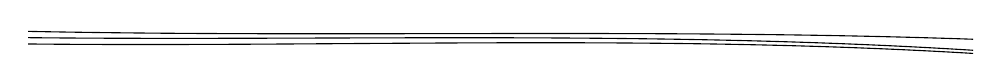
\begin{tikzpicture}\draw (0,.08).. controls (4,0) and (8,.12) .. (12,-.02);\draw (0,0).. controls (4,-.04) and (8,.09) .. (12,-.16);\draw (0,-.08).. controls (4,-.12) and (8,.04) .. (12,-.20);\end{tikzpicture}}

\margin{\begingroup\setbox0=\hbox{5}\hbox{\rlap{\begin{tikzpicture}[overlay,baseline=0pt]\draw[line width=.45pt] (5pt,17pt) .. controls (-10pt,18pt) and (-12pt,-9pt) .. (2pt,-10pt) .. controls (19pt,-12pt) and (21pt,13pt) .. (8pt,17pt);\draw[line width=.35pt] (-6pt,12pt) .. controls (-2pt,13pt) and (1pt,11pt) .. (1pt,9pt);\end{tikzpicture}}\box0}\endgroup{}}
\uline{pg\unsure{45|47}}\quad $\ell\,3$ ss\quad français : beaucoup de ``donc''.

\uline{pg46}\quad Quel est le sens de (5.2.3,1) et de \deleted{\unsure{le|la}} ``par définition'' qui suit --

S'agit-il de pro-objets, ou de schémas.
\margin{\begingroup\setbox0=\hbox{je le dis !}\hbox{\rlap{\begin{tikzpicture}[overlay,baseline=0pt]\draw[gray,line width=.35pt] (\dimexpr\wd0-1pt\relax,16pt) .. controls (-12pt,19pt) and (-10pt,-9pt) .. (6pt,-9pt) .. controls (\dimexpr\wd0+15pt\relax,-9pt) and (\dimexpr\wd0+11pt\relax,17pt) .. (\dimexpr\wd0-2pt\relax,16pt);\draw[gray,line width=.35pt] (\dimexpr\wd0+3pt\relax,13pt) .. controls (\dimexpr\wd0+10pt\relax,16pt) and (\dimexpr\wd0+10pt\relax,11pt) .. (\dimexpr\wd0+6pt\relax,9pt);\end{tikzpicture}}\box0}\endgroup{}}

\uline{pg48}\quad $\ell-4$\quad Pourquoi as-tu barré connexe ?

\deleted{\uline{pg53}\quad 5.7 est une redite pour $\ell\ne p$, et un peu idiot pour $\ell=p$.}\quad (utilisé en 5.15)

\mbox{
\begin{tikzpicture}[overlay]\draw (1.55,.08) ellipse (1.85 and .60);\end{tikzpicture}{\Large ?}\quad \uline{pg56 bis}\quad 5.15 :}
\quad tu n'a plus besoin ici de $\operatorname{car}(k)\ne\ell$

54 quater -- 5.11.\quad seraient plutôt que seront.

\uline{55 ter}\quad $\ell-10$. Il serait honnête de dire que 6.6 utilise $\operatorname{car}(K)=0$, via Tate
\margin{\begingroup\setbox0=\hbox{\shortstack[l]{C'est dit\\dans les hyp\\de 5.13}}\hbox{\rlap{\begin{tikzpicture}[overlay,baseline=0pt]\draw[gray,line width=.35pt] (-5pt,3pt) .. controls (-10pt,23pt) and (-5pt,35pt) .. (13pt,39pt) .. controls (37pt,43pt) and (\dimexpr\wd0+6pt\relax,32pt) .. (\dimexpr\wd0+8pt\relax,10pt) .. controls (\dimexpr\wd0+9pt\relax,-7pt) and (14pt,-9pt) .. (1pt,-7pt) .. controls (-4pt,-5pt) and (-5pt,0pt) .. (-5pt,3pt);\draw[line width=.45pt] (-7pt,5pt) .. controls (3cm,4pt) and (8cm,3pt) .. (12cm,7pt);\draw[line width=.35pt] (-7pt,1pt) .. controls (3cm,0pt) and (8cm,-1pt) .. (12cm,3pt);\draw[line width=.3pt] (-7pt,-4pt) .. controls (3cm,-6pt) and (8cm,-4pt) .. (12cm,-7pt);\end{tikzpicture}}\box0}\endgroup{}}



\margin{\begingroup\setbox0=\hbox{6}\hbox{\rlap{
\begin{tikzpicture}[overlay,baseline=0pt]\draw[line width=.45pt] (-3pt,15pt) .. controls (-12pt,9pt) and (-10pt,-8pt) .. (0pt,-10pt) .. controls (15pt,-11pt) and (22pt,7pt) .. (12pt,16pt) .. controls (7pt,18pt) and (-1pt,18pt) .. (-3pt,15pt) .. controls (-5pt,12pt) and (-5pt,11pt) .. (-5pt,9pt);\end{tikzpicture}}\box0}\endgroup{}}
\uline{pg57/58} : tu supposes tantôt $A^0$ $\ell$-divisible $(58,\ell-11)$, tantôt non $(57,\ell\,3)$

\uline{pg58}\quad $\ell-5$\quad
\mbox{\begin{tikzpicture}[overlay]\draw[gray,line width=.35pt] (.84,-.04) .. controls (.63,.34) and (.94,.63) .. (1.19,.55) .. controls (1.58,.41) and (1.31,-.19) .. (.93,-.13);\end{tikzpicture}$({}_{p^\infty}X)^0$}\quad \begingroup\setbox0=\hbox{?}\hbox{\rlap{\begin{tikzpicture}[overlay,baseline=0pt]\draw[line width=.45pt] (0pt,14pt) .. controls (-9pt,10pt) and (-8pt,-7pt) .. (0pt,-9pt) .. controls (16pt,-11pt) and (21pt,8pt) .. (12pt,15pt) .. controls (8pt,18pt) and (-2pt,18pt) .. (-4pt,13pt);\draw[line width=.35pt] (-4pt,13pt) .. controls (-1pt,18pt) and (2pt,19pt) .. (2pt,15pt);\end{tikzpicture}}\box0}\endgroup{}
\qquad itou plus loin --

\uline{pg\unsure{59|54}}\quad Je ne comprends rien -- Que fais-tu de la partie discrète ? --
\margin{\uline{CANULAR ?}!}

Je ne crois pas que la plus grande \deleted{\unsure{AG|VA}} sous VA ordinaire puisse se relever ($\hat{\mathrm m}$ en cas de bonne réduction).

\uline{ie}\quad 63 est faux (déformer de façon générale $E\times F$, $E$ et $F$ elliptiques, $E$ ordinaire, $F$ non ordinaire ; général $\Rightarrow$ générique simple.

\margin{5}
\normalmarginpar
